\begin{ex}
(Uel) No diagrama a seguir, o espaço amostral S representa um grupo de amigos que farão uma viagem. O conjunto A  indica a quantidade de pessoas que já foram a Maceió e o conjunto B, a quantidade de pessoas que já foram a Fortaleza.
 \begin{center}
  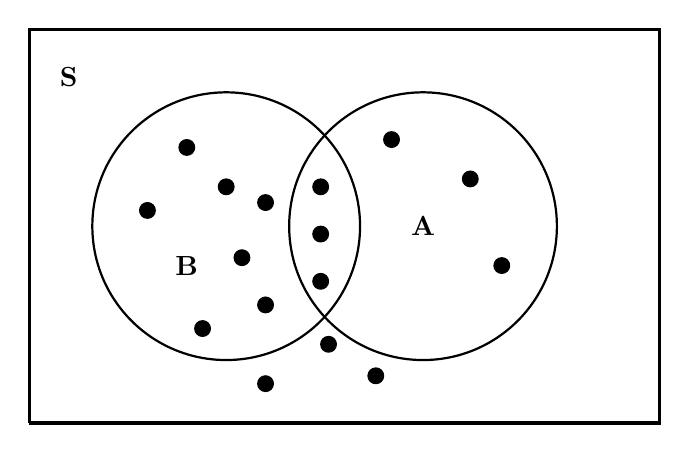
\begin{tikzpicture}
    \draw [very thick] (0,0)--(8,0)--(8,5)--(0,5)--(0,0);
    \draw [thick](2.5,2.5) circle [radius = 1.7];
    \draw [thick](5,2.5) circle [radius = 1.7];
    \draw (2,3.5) [fill] circle [radius = .1];
    \draw (2.5,3) [fill] circle [radius = .1];
    \draw (1.5,2.7) [fill] circle [radius = .1];
    \draw (3,2.8) [fill] circle [radius = .1];
    \draw (2.7,2.1) [fill] circle [radius = .1];
    \draw (3,1.5) [fill] circle [radius = .1];
    \draw (2.2,1.2) [fill] circle [radius = .1];
    \draw (3.7,3) [fill] circle [radius = .1];
    \draw (3.7,2.4) [fill] circle [radius = .1];
    \draw (3.7,1.8) [fill] circle [radius = .1];
    \draw (4.6,3.6) [fill] circle [radius = .1];
    \draw (5.6,3.1) [fill] circle [radius = .1];
    \draw (6,2) [fill] circle [radius = .1];
    \node at (5,2.5) {\textbf{A}};
    \node at (2,2) {\textbf{B}};
    \node at (.5,4.4) {\textbf{S}};
    \draw (3,.5) [fill]circle [radius = .1];
    \draw (3.8,1) [fill]circle [radius = .1];
    \draw (4.4,.6) [fill] circle [radius = .1];
  \end{tikzpicture}
 \end{center} 


A empresa de turismo que está organizando a viagem fará o sorteio de uma passagem gratuita. Considerando que a pessoa sorteada já tenha ido à Fortaleza, assinale a alternativa que indica a probabilidade de que ela também já tenha ido à Maceió.
   \begin{enumerate}[(a)]
   \item 18,75\%
   \item 30\%
   \item 33,33\%
   \item 50\%
   \item 60\%
   \end{enumerate}
     \begin{sol}
       resposta: b \\
       10 pessoas já foram a Fortaleza e 3 já foram a Maceio $\Longrightarrow p=\frac{3}{10}=$30\%
     \end{sol}
\end{ex}